%% Template for SDP report, adapted from mlp_cw2_template, 2018. 

%% Based on  LaTeX template for ICML 2017 - example_paper.tex at 
%%  https://2017.icml.cc/Conferences/2017/StyleAuthorInstructions

\documentclass{article}
\usepackage[T1]{fontenc}
\usepackage{amssymb,amsmath}
\usepackage{txfonts}
\usepackage{microtype}
\usepackage{xspace}
\xspaceaddexceptions{\%}

% Lists with less spacing between items
\usepackage{paralist}

% For figures
\usepackage{graphicx}
\usepackage{subfig} 

% For citations
\usepackage{natbib}

% For algorithms
\usepackage{algorithm}
\usepackage{algorithmic}

% the hyperref package is used to produce hyperlinks in the
% resulting PDF.  If this breaks your system, please commend out the
% following usepackage line and replace \usepackage{mlp2017} with
% \usepackage[nohyperref]{mlp2017} below.
\usepackage{hyperref}
\usepackage{url}
\urlstyle{same}

% Packages hyperref and algorithmic misbehave sometimes.  We can fix
% this with the following command.
\newcommand{\theHalgorithm}{\arabic{algorithm}}


% Set up MLP coursework style (based on ICML style)
\usepackage{mlp2018}
\mlptitlerunning{SDP Demo \demoNumber  Group (\groupNumber)}
\bibliographystyle{icml2017}


\DeclareMathOperator{\softmax}{softmax}
\DeclareMathOperator{\sigmoid}{sigmoid}
\DeclareMathOperator{\sgn}{sgn}
\DeclareMathOperator{\relu}{relu}
\DeclareMathOperator{\lrelu}{lrelu}
\DeclareMathOperator{\elu}{elu}
\DeclareMathOperator{\selu}{selu}
\DeclareMathOperator{\maxout}{maxout}







%% You probably do not need to change anything above this comment

%% REPLACE the details in the following commands with your details
\setGroupNumber{1}
\setGroupName{My Group}
\setProductName{My Product}
\setDemoNumber{1}
\setLogoFileName{figs/sdp_logo_placeholder.png}

\begin{document} 

\makeSDPTitle{Demo}

% Previous MLP Style Title Layout working. 
% \twocolumn[
    % \mlptitle{\productName: SDP Demo \demoNumber}
    % \centerline{Group \groupNumber: \groupName}
% ]

\begin{abstract} 
The abstract should consist of one sentence describing the intended functionality of your system, followed by a few sentences (100--200 words) summarising the key advances made for this demo. This should give the reader a clear expectation of what will be demonstrated. This report will not be read by the experts that will judge you during demo days.
\end{abstract} 

\section*{Introduction}
\label{sec:intro}
This document provides a template for the SDP demo report.  This template structures the report into sections, which you are required to use. You can change the subsection headings if you wish. In this template the text in each section will include an outline of what you should include in each section, along with some practical LaTeX examples (for example figures, tables, algorithms).  Your document should be no longer than \textbf{3 pages} for the first demo, \textbf{4} for the second demo and \textbf{6} for the final demo. You can include a bibliography and an Appendix with no length restrictions but you won't have the guarantee that it will be read. 

The logo, group number, product name and team name should be updated accordingly in the template. You should also update the demo number header in the template (see line 11 in the source).

You should delete this introduction section (no introduction is required).

\section{Project management update} 

The following items are expected in this section

\begin{enumerate}
    \item This section should start with your goals:
\begin{itemize}
    \item Use a bullet point list to indicate each of the goals you had set for this demo, appended with "achieved", "partly achieved" "not achieved".
\end{itemize}


\item Concisely summarise the reasons for any deviations from achievement of your intended goals.

\item Provide a description of how your group organised the work towards the goals. Highlight any methods used to ensure effective group work such as protocols for code integration, task tracking, automated testing, etc. Copy and paste from your own previous reports is authorised but should be clearly indicated using text colours.

\item Provide an overview of which teams members worked on which aspects, and account for the total number of hours spent by each team member on the project so far.

\item Provide a summary of how the budget allocated to your team (both technician time and money) has been spent so far.

\item Provide a clear statement of any modification (relative to your original plan) that you wish to make to your goals for the next demonstration, with the appropriate justification.

\end{enumerate}

\subsection*{Demo 3 instructions}
For the final report, this section should follow the same structure, but provide a synthesis of the whole project rather than just focusing on what happened since demo 2. 

Item 1 should only list partially achieved / unachieved tasks in the project.

Item 6 should be replaced by a concise post-mortem on what went well and wrong during the project.


\section{Quantitative analysis and testing}

This Section provides a clear summary of the tests designed and run to prove the reliability of the code / system as a whole, with details allowed in the appendix.  

This section should first outline any testing methods you used (e.g. repeated runs of subsystems, data-logging, naive user testing). 

It should then present relevant quantitative results. If you are using graphs, please make sure they are properly labelled and logically illustrate the point you want to make (e.g. to compare two algorithms).

For each test, the following points should be answered:

\begin{itemize}
    \item Relevance: How is the test relevant to the system (what does the outcome demonstrate)? How does the outcome of the test allows to validate a milestone / affects the project plan ?
    \item Interpretation: What do the actual results say about the system and why (eg. does a 72\% success rate on a classification algorithm mean that the system is robust or on the contrary that it is not)?
    \item Robustness: is the test exhaustive / are all edge cases considered?
\end{itemize}


At an absolute minimum, this section should provide a table (for instance, table~\ref{tab:sample-table}, using the \verb+table+ environment) of success rates for repeated runs of the whole system.

\begin{table}[h]
\vskip 3mm
\begin{center}
\begin{small}
\begin{sc}
\begin{tabular}{lcccr}
\hline
\abovespace\belowspace
Test  & Time(mins) & Errors & Success \\
\hline
\abovespace
1    & 1:30 & 0 & $\surd$ \\
2    & 3:00 & 2 & $\times$\\
3    & 2:20 & 1 & $\surd$ \\
4    & 1:50 & 1 & $\times$\\
\belowspace
5    & 2:10 & 0 & $\surd$ \\
\hline
\end{tabular}
\end{sc}
\end{small}
\caption{Results for 5 tests of the system.}
\label{tab:sample-table}
\end{center}
\vskip -3mm
\end{table}

If you need a figure or table to stretch across two columns use the \verb+figure*+ or \verb+table*+ environment instead of the \verb+figure+ or \verb+table+ environment.  Use the \verb+subfigure+ environment if you want to include multiple graphics in a single figure.

\subsection*{Demo 3 instructions}
In your final report all the updated relevant tests that were performed during the project should be presented and accordingly commented.
The final version of this section should convince the reader of the validity of the decisions made and the reliability of the system.

\section{Budget}
Each report should contain an actualization of the estimated total budget 
of your system.

\section{Miscellaneous}
This optional section includes any description of work that seems of relevance to the team. It can be the result of a user study, a commercialisation analysis, the description of a clever algorithm / specific solution to a problem etc.

This section should remain short and be completed if necessary with an appendix.

Pictures should be used if appropriate (for instance, figure~\ref{fig:sample-fig}), using the \verb+\includegraphics+ environment to include an image (pdf, png, or jpg formats), ideally with informative labels added. 

To keep your folders clean, it is often a good idea to keep your images in a separate folder. In this example, we've put the figures in the \texttt{figs/} folder. To include images from different folders, give the relative path from this file. Example: \verb+\includegraphics{figs/image_filename}+.

\begin{figure}[tb]
\vskip 5mm
\begin{center}
\centerline{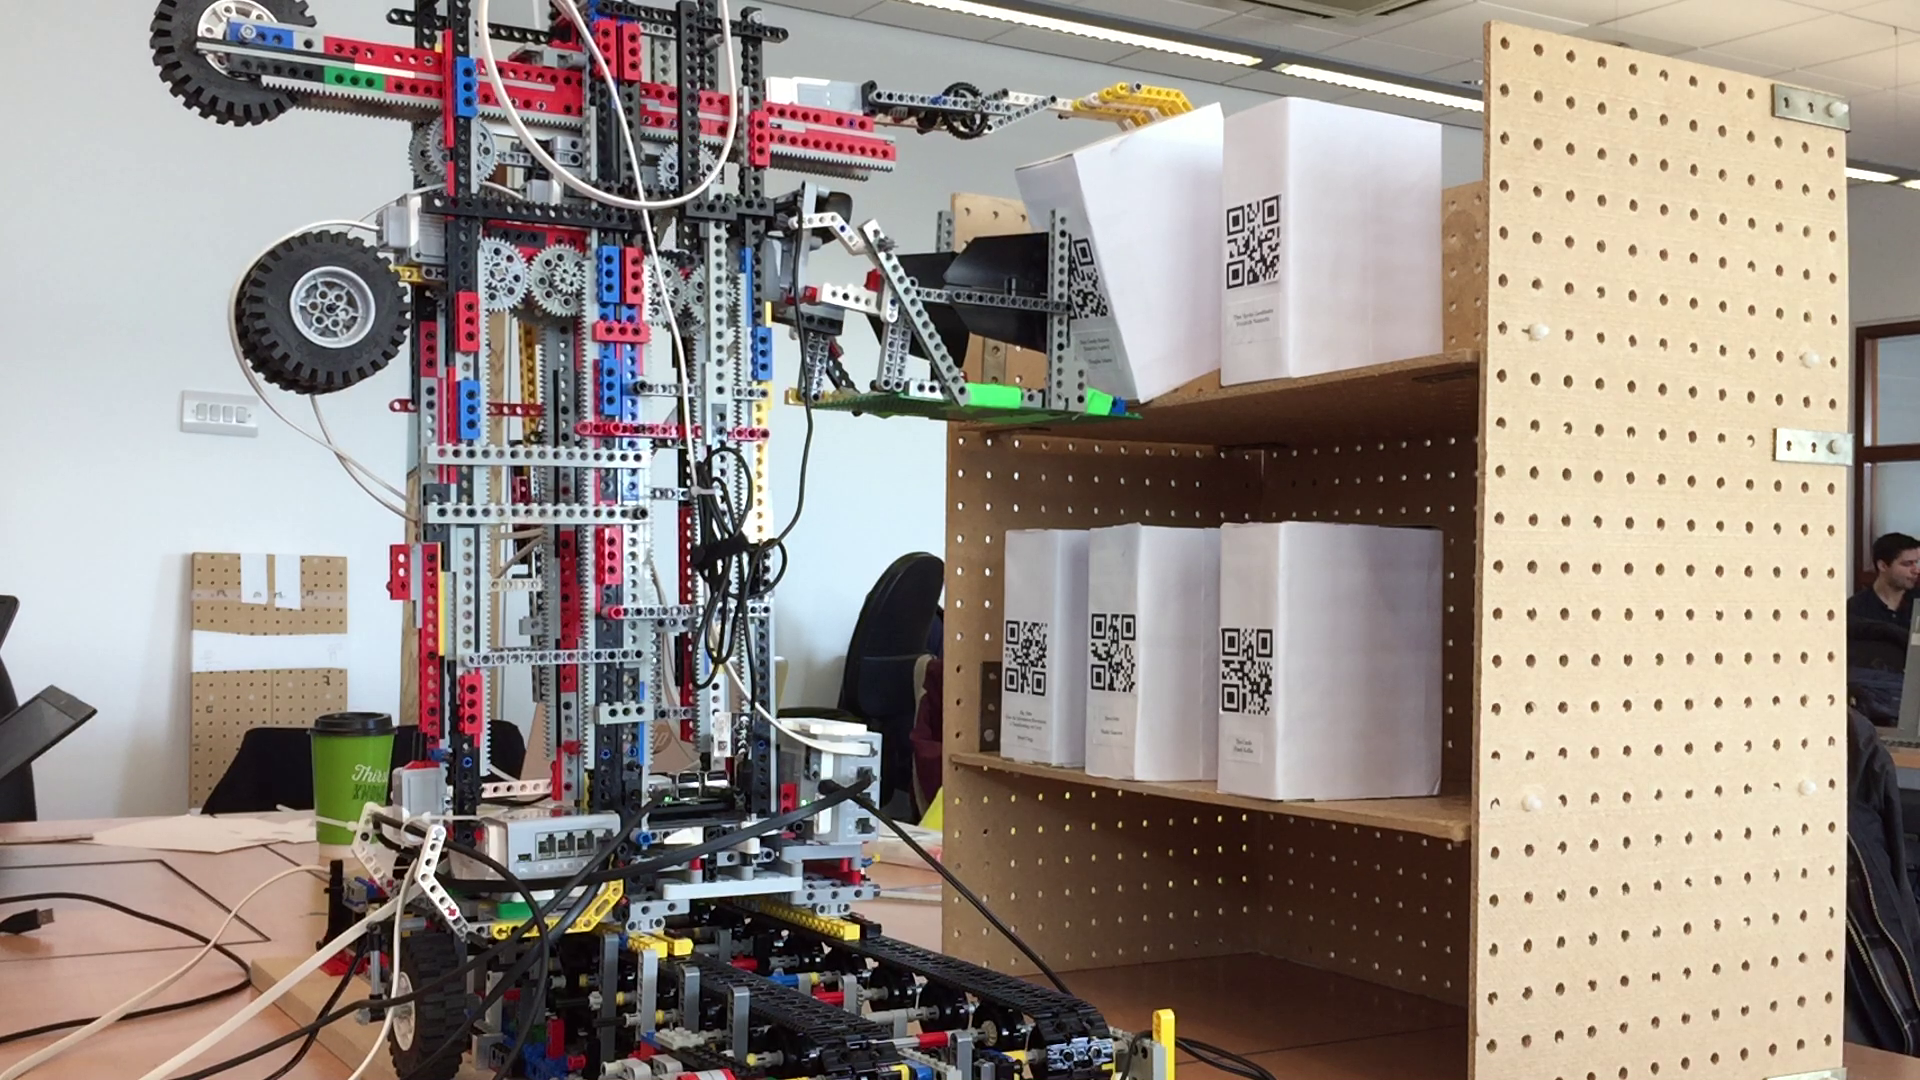
\includegraphics[width=\columnwidth]{figs/crane}}
\caption{Lego construction: highlight any salient features in the caption}
\label{fig:sample-fig}
\end{center}
\vskip -5mm
\end{figure} 

If you present algorithms, you can use the \verb+algorithm+ and \verb+algorithmic+ environments to format pseudocode (for instance, Algorithm~\ref{alg:example}). These require the corresponding style files, \verb+algorithm.sty+ and \verb+algorithmic.sty+ which are supplied with this package. 

\begin{algorithm}[ht]
\begin{algorithmic}
   \STATE {\bfseries Input:} data $x_i$, size $m$
   \REPEAT
   \STATE Initialize $noChange = true$.
   \FOR{$i=1$ {\bfseries to} $m-1$}
   \IF{$x_i > x_{i+1}$} 
   \STATE Swap $x_i$ and $x_{i+1}$
   \STATE $noChange = false$
   \ENDIF
   \ENDFOR
   \UNTIL{$noChange$ is $true$}
\end{algorithmic}
  \caption{Bubble Sort}
  \label{alg:example}
\end{algorithm}

You can also include references to scientific papers \cite{langley00} or studies that will help justifying the value / interest of your system or validate a specific design choice.

\section*{Submission}
This section is to be deleted.

The document should be submitted on Learn by one group member.
The filename must be  \verb|group-[g]-demoX.pdf| where \verb|[g]| is the group number and again  \verb|X| is the demo number.
This document should be submitted by a group member nominated for this purpose, and also emailed to the group mentor at the time of submission.


\appendix

\section{Appendix}
The optional Appendix should complement the report. An updated Gantt Chart might be relevant. It could also include a developed analysis of a conducted user study or the details of a nice algorithm. 

%% Include any references in a bibliography

\bibliography{example-refs}

\end{document} 

